\documentclass[12pt,a4paper]{article}
\usepackage[utf8]{inputenc}
\usepackage{amsmath}
\usepackage{amsfonts}
\usepackage{amssymb}
\usepackage{makeidx}
\usepackage[left=0.50cm, right=0.50cm, top=0.50cm, bottom=0.50cm]{geometry}
\author{fofo}
\usepackage{pgfplots}

% The data files, written on the first run.


\begin{document}

In Fig.\ref{fig:ProClamping}, from 6 to 9 and from 16 to 20, the subway is in the {\em Rush Hours}. During rush hours, the probability for doors clamping is 0.4. The normal hours are from 5 to 6, from 9 to 16, and from 20 to 22, the probability is 0.25.

\begin{figure}
\centering
\scalebox{1}[1]{
\pgfplotsset{grid style={dashed}}
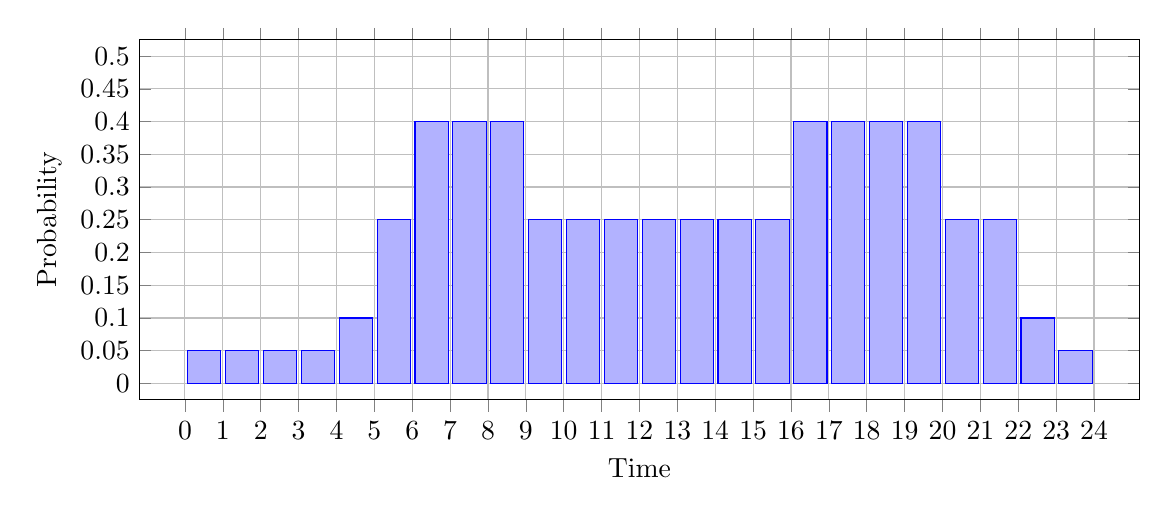
\begin{tikzpicture}
\begin{axis}[grid=major,
scale only axis,
    ybar,
    bar shift=7pt,
    bar width=12pt,
    width=5in,height=1.8in,
    ymin=0.0,ymax=0.50 ,
    xmin=0, xmax=24,
    enlargelimits=0.05,
    ylabel={Probability},
    xlabel={Time},
    symbolic x coords={0,1,2,3,4,5,6,7,8,9,10,11,12,13,14,15,16,17,18,19,20,21,22,23,24},
    xtick={0,1,...,24},
    ytick={0,0.05,...,0.5},
    %nodes near coords,
    nodes near coords align={vertical},
    y tick label style={/pgf/number format/.cd,%
              scaled y ticks = false,
              set thousands separator={},
              fixed,},
    ]
\addplot coordinates {
(0,0.05)
(1,0.05)
(2,0.05)
(3,0.05)
(4,0.1)
(5,0.25)
(6,0.4)
(7,0.4)
(8,0.4)
(9,0.25)
(10,0.25)
(11,0.25)
(12,0.25)
(13,0.25)
(14,0.25)
(15,0.25)
(16,0.4)
(17,0.4)
(18,0.4)
(19,0.4)
(20,0.25)
(21,0.25)
(22,0.1)
(23,0.05)
};
\end{axis}
\end{tikzpicture}
}
\caption{The Probabilities for Clamping for All Time in A Day}
\label{fig:ProClamping}
\end{figure}

\begin{figure}[tbph]
\centering
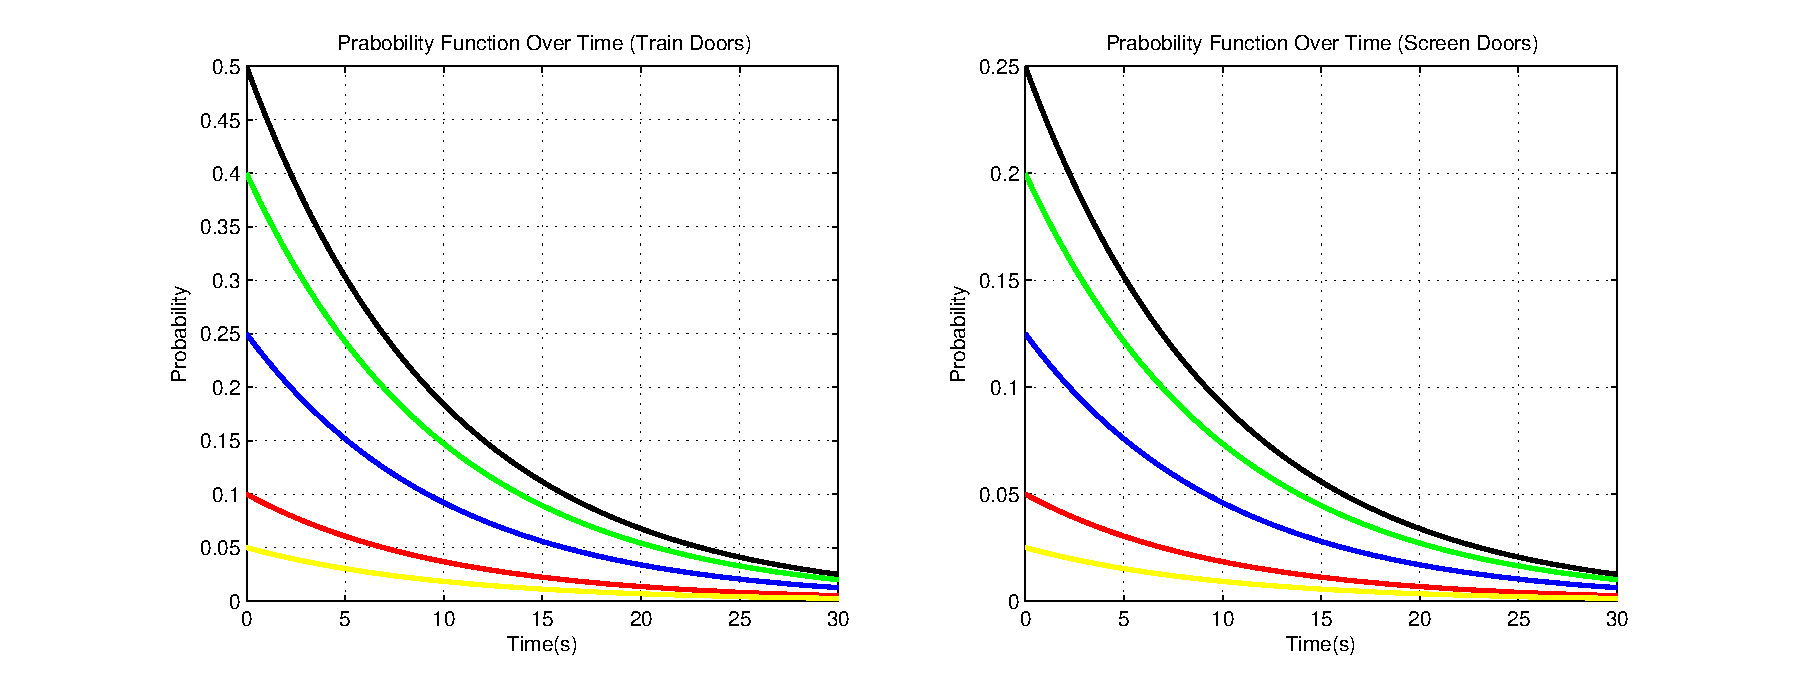
\includegraphics[width=1.0\linewidth]{./figures/ProbabilityOverTimeFigure}
\caption{The variation of probability for doors clamping during the closing.}
\label{fig:ProbabilityOverTimeFigure}
\end{figure}
In Fig.\ref{fig:ProbabilityOverTimeFigure}, for one duration, we suppose that the highest probability of doors clamping for the train doors is 0.5 (the black one in Fig.\ref{fig:ProbabilityOverTimeFigure}), and, as the screen doors are closed after train doors, the probability of doors clamping for screen doors is smaller (e.g., 0.25) than the probability for train doors.
During doors closing, the probability  of doors clamping will decrease with time.

\begin{tikzpicture}
\draw (0,0) node {.};
\draw (15,0) node {.};
\end{tikzpicture}
\end{document}